\chapter{Dasar Teori}
\label{chap:teori}
Bab ini berisi dasar teori dari pembangunan Aplikasi Pencarian Rute Kendaraan Umum untuk Windows Phone. Beberapa teori yang dibahas dalam bab ini  adalah XAML, kontrol terhadap ponsel, siklus hidup Windows Phone, peta, lokasi , pemanfaatan sumber data, dan Kiri API. 

% Windows Phone
\section{Windows Phone}
\label{sec:Windows Phone}
\hspace{0.5cm} Windows Phone merupakan sistem operasi untuk perangkat bergerak yang dikembangkan Microsoft. Pengembangan aplikasi Windows Phone membutuhkan Windows Desktop 8 sebagai media pengembangan. Bahasa pemrograman yang digunakan untuk membuat perangkat lunak di Windows Phone yaitu C\# atau Visual Basic\cite{Manning}.  

Pada sub bab~\ref{subsec:Lingkungan Kerja} sampai~\ref{subsec:Memanfaatkan Sumber Data} akan membahas pemrograman di Windows Phone. Pembahasan akan dimulai dengan apa itu Windows Phone dan fitur di Windows Phone yang akan digunakan dalam pembangunan perangkat lunak Pencarian Rute Kendaraan di Windows Phone. 

% SUB Lingkungan Kerja
\subsection{Lingkungan Kerja}
\label{subsec:Lingkungan Kerja}
\hspace{0.5cm} Microsoft .NET framework merupakan sebuah perangkat lunak yang dibangun untuk membantu dalam pembangunan aplikasi di Windows, Windows Phone, Windows Server, and Microsoft Azure\cite{MSDN}. Microsoft .NET framework terdiri dari runtime bahasa umum dan perpustakaan kelas .NET Framework, yang meliputi kelas, interface, dan jenis nilai yang mendukung berbagai teknologi. Microsoft .NET Framework menyediakan lingkungan yang mudah dikelola, pengembangan yang disederhanakan, dan integrasi dengan berbagai bahasa pemrograman, termasuk Visual Basic dan Visual C\#.

Seperti yang telah disebutkan ada dua bahasa pemrograman dalam .NET Framework yang dipakai dalam pembangunan aplikasi di Windows Phone 8 yaitu Visual Basic dan Visual C\#. \newline Untuk masalah kehandalan keduanya menawarkan kehandalan yang baik. Kelebihan dari Visual Basic adalah bahasa pemrograman berorientasi objek yang kuat dan memiliki banyak pengenbangan fitur di inheritance, polymorphism, interfaces, and overloading\cite{MSDN}. Kelebihan dari C\# yang merupakan pengembangan dari C/C++ adalah sederhana, modern, aman dan berorientasi objek\cite{MSDN}. Satu hal yang dirasakan penulis adalah kenyamanan ketika memilih bahasa .NET tersebut. Akan lebih mudah bagi developer yang menggunakan Visual Basic 6.0  untuk menggunakan Visual \newline Basic .NET. Tetapi bagi  developer yang menggunakan C++ atau java sebelumnya akan lebih mudah menggunakan C\#.
%kutipan mengenai .NET
%\footnotetext[2]{\url{http://msdn.microsoft.com/en-us/library/vstudio/w0x726c2\%28v=vs.110\%29}}
%\footnotetext[3]{\url{http://msdn.microsoft.com/en-us/library/aa903378\%28v=vs.71\%29.aspx}}
%\footnotetext[4]{\url{http://msdn.microsoft.com/en-us/library/aa287558\%28v=vs.71\%29.aspx}}

% SUB Mengenai XAML
\subsection{XAML}
\label{subsec:XAML}
\hspace{0.5cm} \textit{Extensible Application Markup Language} (XAML) merupakan bahasa deklaratif yang dipakai untuk membuat antarmuka aplikasi. XAML merupakan bahasa yang digunakan untuk membuat antarmuka di Windows Phone 8\cite{Manning}. Pada dasarnya penggunaan XAML sama dengan HTML pada pembuatan antarmuka web. XAML dapat menginisialisasi objek dan mengatur properti untuk menunjukan hubungan antar objek.

Untuk aturan penulisan sintak XAML didasarkan pada XML. Setiap XAML Windows Runtime menggunakan konvensi bahasa XAML dan ditulis pada \textit{namespace} yang ditandai dengan \textit{prefix} x sebagai elemen paling atas. Setelah itu di baris ke dua dimulai dengan xmlns diikuti titik dua, lalu nama dari \textit{namespace}, diikuti tanda sama dengan dan \textit{path} yang merepresentasikan \textit{namespace}.
\textit{Prefix} x pada XAML mengandung beberapa struktur program yang sering kita gunakan yaitu :
\begin{itemize}
	\item x:Key : sebuah nama unik untuk menunjuk referensi ke suatu resource atau berkas lain. Nilai ini dapat dipanggil kembali untuk menggunakan resource tersebut.
	\item x:Class : menunjukkan nama kelas.
	\item x:Name : menunjukkan nama sebuah obyek dan untuk membedakan antar obyek yang satu dengan obyek yang lain.
	\item x:Uid : mengidentifikasi elemen objek dalam XAML. Elemen objek merupakan objek yang dapat melakukan kontrol terhadap kelas atau elemen lain yang ditampilkan di desain antarmuka.
\end{itemize}	

% SUB Mengenai Kontrol terhadap Ponsel
\subsection{Kontrol terhadap Ponsel}
\label{subsec:Kontrol terhadap Ponsel}
\hspace{0.5cm} Maksud dari kontrol terhadap ponsel adalah pengaturan tata letak terhadap antarmuka di Windows Phone\cite{MSDN}. Windows Phone 8 menyediakan banyak set kontrol yaitu tata letak, tombol, kontrol masukan untuk mendapatkan informasi sampai ke menu. 

% SUBSUB Navigasi
\subsubsection{Navigasi}
\label{subsubsec:Navigasi}
\hspace{0.5cm} Aplikasi yang dibuat di Windows Phone didasarkan pada model halaman. Model halaman adalah pengguna berpindah dari satu halaman ke halaman lain dengan konten yang berbeda dan \textit{frame} sebagai pengontrolnya. Setiap antarmuka aplikasi dibungkus dengan \textit{frame}. \textit{Frame} ini yang akan melakukan kontrol terhadap aplikasi dan memungkinkan perpindahan dari satu halaman ke halaman lain. Sedangkan halaman merupakan pembungkus dari elemen di dalamnya saja. Untuk lebih jelas mengenai \textit{frame}, halaman, dan area konten dapat dilihat pada gambar~\ref{fig:nav_hierarchy}.

\begin{figure}[h]
	\centering
		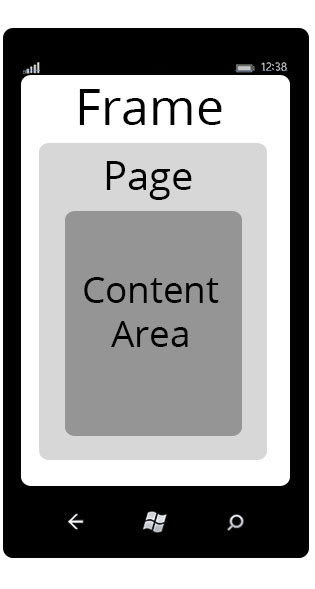
\includegraphics[scale=0.5]{Gambar/nav_hierarchy}
	\caption{Hirarki Navigasi}
	\label{fig:nav_hierarchy}
\end{figure}

\newpage
% SUBSUB Mengenai Tata Letak
\subsubsection{Kontrol Tata Letak}
\label{subsubsec:Kontrol Tata Letak}
\hspace{0.5cm} Kontrol tata letak merupakan penampung pada antarmuka Windows Phone untuk objek di antarmuka dan kontrol yang lain (tombol radio, \textit{textbox}, dan lain-lain). Kontrol tata letak digunakan untuk meletakan objek-objek di layar. Ketika pertama membuat aplikasi Windows Phone maka tata letak dasar sebagai penampung akan langsung dibuat berikut panel judul dan panel konten. Selanjutnya untuk penambahan kontrol tata letak yang lain dapat ditambahkan di panel konten.


Terdapat 3 jenis panel yang digunakan untuk menangani tata Letak yaitu \textit{Grid}, \textit{StackPane}, dan \textit{Canvas}. Perlu diperhatikan bahwa setiap halaman hanya memiliki satu jenis panel. Berikut adalah 3 jenis panel pada Windows Phone:

\begin{itemize}
	\item \textit{StackPanel} merupakan panel yang memposisikan element menjadi 1 baris dan beberapa elemen di setiap halaman diposisikan horizontal atau vertical saja.
	\item \textit{Grid} merupakan panel yang mendukung tata letak yang rumit. Panel ini memposisikan elemen di baris dan kolom mana saja di setiap halaman.
	\item \textit{Canvas} memposiskan elemen sebagai absolut kordinat. Jadi setiap elemen di dalam \textit{canvas} dapat diposisikan spesifik sesuai kordinat x dan y.
\end{itemize}

Kode untuk mengatur jenis panel pada Windows Phone dapat dilihat pada \textit{listing}~\ref{lst:grid}.
\begin{lstlisting} [caption= {Kode Tata Letak Grid},label={lst:grid}]
	<Grid x:Name="ContentPanel">
	</Grid>
\end{lstlisting}
	
% SUBSUB Mengenai Kontrol Masukan
\subsubsection{Kontrol Terhadap Teks}
\label{subsubsec:Kontrol Terhadap Teks}
\hspace{0.5cm} Kontrol terhadap teks  akan menampilkan konten yang memiliki tipe \textit{String}. Terdapat berbagai macam kontrol terhadap teks di Windows Phone yaitu \textit{TextBlock}, \textit{TextBox} dan \textit{PasswordBox}. Ketiga macam kontrol tersebut dibedakan berdasarkan tujuannya. Berikut keterangan, gambar~\ref{fig:kontrol_teks}, dan kode pada \textit{listing}~\ref{lst:text} kontrol teks.

\begin{itemize}
	\item \textit{TextBlock} merupakan tempat menaruh potongan teks yang hanya bisa dilihat.
	\item \textit{TextBox} biasanya digunakan untuk teks masukan yang pendek. Tapi bisa juga dipakai untuk masukan yang banyak dan beberapa baris.
	\item \textit{PasswordBox} biasanya digunakan untuk masukan yang bersifat rahasia. Karakter yang dimasukan langsung disamarkan menjadi bentuk titik.
\end{itemize}

\begin{figure}[h]
	\centering
		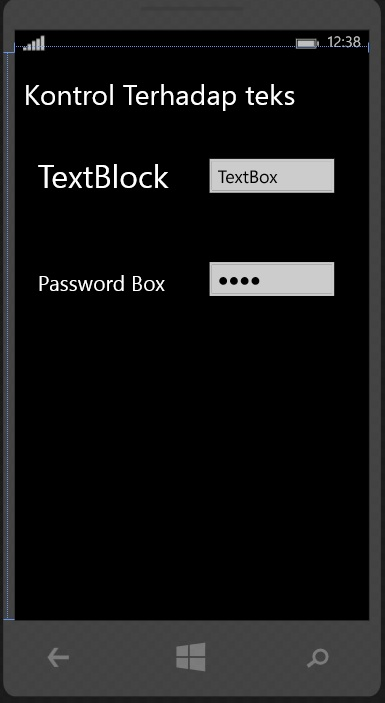
\includegraphics[scale=0.5]{Gambar/Tombol/kontrol_teks}
	\caption{\textit{TextBlock}, \textit{TextBox} dan \textit{PasswordBox}}
	\label{fig:kontrol_teks}
\end{figure}

\begin{lstlisting} [caption= {Kode untuk Menampilkan \textit{TextBlock} dan \textit{TextBox}},label={lst:text}]
	<TextBlock x:Name="TextBlock1" Text="TextBlock"/>
	<TextBox x:Name="TextBox1"Text="TextBox"/>
\end{lstlisting}

% SUBSUB Mengenai Kontrol Masukan
\subsubsection{Tombol dan Kontrol Pilihan}
\label{subsubsec:Tombol dan Kontrol Pilihan}
\hspace{0.5cm} Tombol memungkinkan pengguna untuk berpindah halaman. Sedangkan kontrol pilihan memudahkan dalam memilih. Berikut keterangan, gambar~\ref{fig:kontrol_tombol}, dan kode pada \textit{listing}~\ref{lst:tombol} tombol dan kontrol pilihan.
 
\begin{itemize}
	\item \textit{Button} merupakan kontrol yang dipakai pengguna untuk mengaktifkan \textit{event} tekan.
	\item \textit{HyperlinkButton} merupakan kontrol yang menampilkan tautan. Jika \textit{HyperlinkButton} ditekan maka akan berpindah ke halaman yang akan dituju.	
	\item \textit{CheckBox} merupakan kontrol yang memungkinkan pengguna memilih beberapa item.
	\item \textit{RadioButton} merupakan kontrol yang memungkinkan pengguna memilih satu pilihan dari beberapa pilihan.
	\item \textit{Slider} merupakan kontrol yang memungkinkan pengguna memilih nilai kisaran dari jalur yang sudah disediakan.
\end{itemize}

\begin{figure}[h]
	\centering
		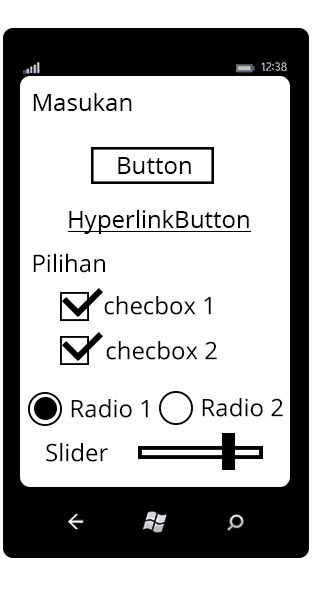
\includegraphics[scale=0.5]{Gambar/Tombol/tombol_dan_pilihan}
	\caption{Gambar Kontrol pada Windows Phone}
	\label{fig:kontrol_tombol}
\end{figure}

\begin{lstlisting} [caption= {Kode untuk Menampilkan \textit{TextBlock}, \textit{TextBox}, dan \textit{PasswordBox}},label={lst:tombol}]
	<Button x:Name="find" Content="Button"/>
\end{lstlisting}

% SUBSUB Kontrol Daftar
\subsubsection{Kontrol Daftar}
\label{subsubsec:Kontrol Daftar}
\hspace{0.5cm} Kontrol yang dipakai untuk menampilkan daftar dari beberapa \textit{item}. Berikut keterangan, gambar~\ref{fig:antarmukaListBox}, dan kode pada \textit{listing}~\ref{lst:listBox} kontrol daftar. 

\begin{itemize}
	\item \textit{ListBox} akan menampilkan daftar \textit{item}. Daftar ini dapat dipilih dengan cara ditekan.
	\item \textit{LongListSelector} dipakai untuk mengelompokan, menampilkan, dan melakukan penggulungan terhadap daftar yang panjang.
\end{itemize}

\newpage

\begin{figure}[h]
	\centering
		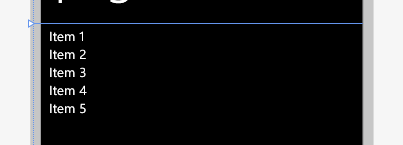
\includegraphics[scale=0.4]{Gambar/kontrol/listBox.PNG}
	\caption{Antarmuka \textit{ListBox}}
	\label{fig:antarmukaListBox}
\end{figure}

\begin{lstlisting} [caption= {Kode untuk menampilkan \textit{listBox}},label={lst:listBox}]
	<ListBox>
		<ListBoxItem Content="Item 1" />
		<ListBoxItem Content="Item 2" />
		<ListBoxItem Content="Item 3" />
		<ListBoxItem Content="Item 4" />
		<ListBoxItem Content="Item 5" />
	</ListBox>
\end{lstlisting}

% SUB Mengenai Siklus Hidup Aplikasi
\subsection{Siklus Hidup Aplikasi}
\label{subsec:Siklus Hidup Aplikasi}
\hspace{0.5cm} Siklus hidup aplikasi merupakan waktu mulai dari aplikasi dijalankan sampai dengan aplikasi diberhentikan dari memori. Siklus hidup aplikasi penting diketahui agar pengguna tidak kecewa (dalam aplikasi ini yaitu kecewa karena aplikasi keluar saat layar perangkat dimatikan) menggunakan aplikasi serta memastikan sumber daya tersedia (dalam aplikasi ini yaitu sumber daya GPS). Seringkali pengguna tidak berhati-hati dalam menggunakan aplikasi, maka dari itu penulis harus memahami kapan aplikasi harus diaktifkan, ditangguhkan, atau bahkan dinonaktifkan karena sudah tidak digunakan. Gambar~\ref{fig:Siklus Hidup Aplikasi} adalah ilustrasi dari siklus hidup pada Windows Phone.

\begin{figure}[h]
	\centering
		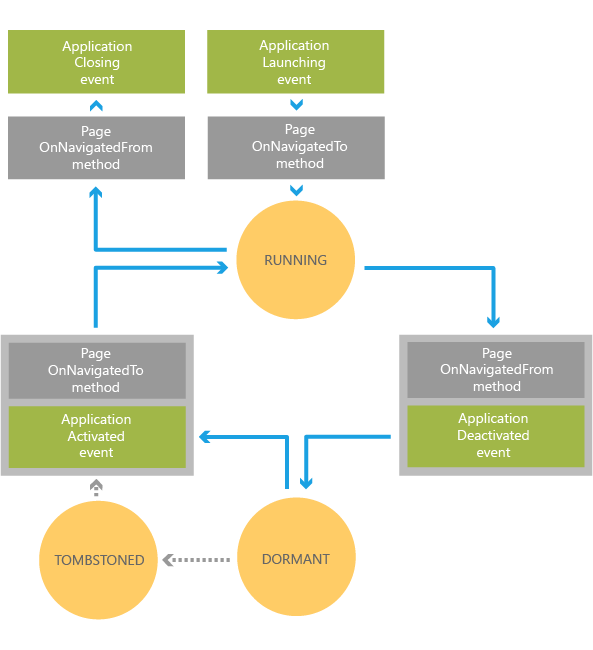
\includegraphics[scale=0.4]{Gambar/lifecycle_wp8}
	\caption{Gambar siklus Hidup Aplikasi\cite{MSDN}}
	\label{fig:Siklus Hidup Aplikasi}
\end{figure}
%sumber http://msdn.microsoft.com/en-us/library/windows/apps/ff817008%28v=vs.105%29.aspx

Sesuai gambar~\ref{fig:Siklus Hidup Aplikasi} lingkaran melambangkan keadaan aplikasi, persegi panjang menunjukan peristiwa aplikasi atau tingkat peristiwa di halaman. Berikut ini adalah keterangan untuk siklus hidup Windows Phone pada gambar~\ref{fig:Siklus Hidup Aplikasi}. 
\begin{itemize}
	\item \textit{The Launching Event} \\
	Merupakan tampilan awal saat aplikasi dipilih yang memberitahukan pengguna bahwa aplikasi sedang dijalankan. \textit{Event} ini akan dipanggil ketika aplikasi di jalankan pertama kali. \textit{Event} ini akan berjalan di belakang (\textit{background processing}) ketika aplikasi ditutup sementara atau sedang berada pada keadaan \textit{Dormant} atau \textit{Tombstoned} menjadi \textit{running}.
	\item \textit{Running} \\
	Setelah dijalankan, aplikasi akan masuk ke keadaan \textit{running}. Hal ini akan terus berlangsung sampai pengguna berpindah ke halaman depan, atau mundur melewati halaman utama aplikasi. Aplikasi keluar dari keadaan \textit{running} jika perangkat di kunci. Keadaan \textit{running} masih dapat terjadi saat perangkat di kunci dengan menonaktifkan \textit{idle detection} pada aplikasi.
	\item \textit{method} \textit{OnNavigatedFrom} \\
	Merupakan \textit{method} yang dipanggil ketika berpindah ke halaman lain aplikasi. Ketika \textit{method} ini dipanggil maka aplikasi akan menyimpan keadaan dari halaman sebelum ditinggalkan. Hal tersebut dibutuhkan agar halaman tersebut bisa dikembalikan ke keadaan sebelum ditinggalkan saat pengguna ingin kembali ke halaman tersebut. Pemanggilan dilakukan ketika berpindah antara halaman di aplikasi atau ketika berpindah aplikasi.
	\item \textit{The Deactivated Event} \\
	\textit{Event} ini akan terjadi ketika pengguna berpindah aplikasi dan menekan tombol "\textit{start}" atau menjalankan aplikasi lain. Untuk penanganan \textit{deactivated event}, aplikasi harus menyimpan data sebelumnya, sehingga data sebelumnya dapat dikembalikan suatu saat. Windows Phone 8 juga mendukung sistem pengembalian data dengan \textit{State Object}. \textit{State Object} akan digunakan untuk menyimpan keadaan aplikasi sebelum aplikasi dinonaktifkan. 
	\item \textit{Dormant} \\
	Keadaan ini akan terjadi setelah \textit{deactivated event}. Pada keadaan ini, semua \textit{thread} aplikasi akan dihentikan dan tidak ada proses yang terjadi, tetapi kondisi aplikasi tetap utuh di memori. Tetapi jika sistem operasi membutuhkan memori yang lebih besar maka aplikasi yang dalam keadaan \textit{Dormant} akan menjadi \textit{Tombstone} untuk membebaskan memori.
	\item \textit{Tombstoned} \\
	Aplikasi yang masuk ke keadaan \textit{Tombstoned} akan dihentikan, namun sistem operasi akan menyimpan informasi aplikasi pada saat aplikasi berada di keadaan \textit{deactivated}.
	\item \textit{The Activated Event} \\
	\textit{Event} ini dipanggil ketika aplikasi meninggalkan keadaan \textit{Dormant} atau \textit{Tombstoned}. Operasi ini dilakukan pada latar belakang. 
	\item \textit{The OnNavigatedTo Method} \\
	\textit{method} ini dipanggil ketika pengguna berpindah ke halaman yang sebelumya ditinggalkan. \textit{method} ini akan memeriksa keadaan aplikasi dan memulihkannya jika keadaan sebelumnya pernah disimpan. 
	\item \textit{The Closing Event} \\
	\textit{Event} ini akan tercapai ketika pengguna berpindah mundur keluar dari halaman utama. Pada kasus ini, aplikasi akan dihentikan dan tidak ada keadaan yang disimpan. 
\end{itemize}

% SUB Peta di Windows Phone
\subsection{Peta di Windows Phone}
\label{subsec:Peta di Windows Phone}
\hspace{0.5cm} Peta yang dipakai di Windows Phone adalah \textit{Windows Phone Maps}. Windows Phone menawarkan beberapa pilihan dalam tampilan peta mulai dari \textit{cartographic}, pencahayaan dan pandangan. Selain tampilan pada sub bab ini akan dibahas mengenai mendapatkan lokasi, petunjuk arah, \textit{MapPolyline} dan \textit{Pushpin}\cite{MSDN}.

% SUBSUB Mengenai Penambahan Peta Ke Aplikasi
\subsubsection{Penambahan Peta Ke Aplikasi}
\label{subsubsec:Penambahan Peta Ke Aplikasi}
\hspace{0.5cm} Untuk penambahan peta pada Windows Phone menggunakan kontrol peta. Kontrol peta merupakan bagian dari \textit{library} Windows Phone. Dengan begitu untuk dapat menggunakannya perlu direferensikan. Untuk dapat menggunakannya juga harus ditambah \textit{capability} ID\_CAP\_MAP. Setelah hal tersebut dilakukan barulah peta dapat ditampilkan. Berikut gambar~\ref{fig:peta}, kode XAML pada \textit{listing}~\ref{lst:mapXAML}, dan kode program pada \textit{listing}~\ref{lst:mapCode} peta.

\begin{figure}[h]
	\centering
		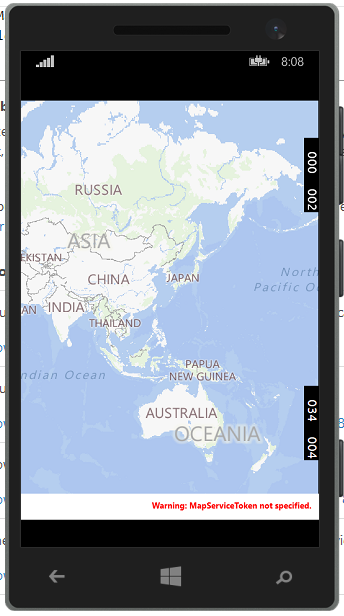
\includegraphics[scale=0.1]{Gambar/map}
	\caption{Tampilan Peta pada Windows Phone}
	\label{fig:peta}
\end{figure}

\begin{lstlisting} [caption= {Menampilkan Peta dengan Nama MyMap dari XAML},label={lst:mapXAML}]
	<Controls:Map x:Name="MyMap"/>
\end{lstlisting}

\begin{lstlisting} [caption= {Menampilkan Peta dengan Nama MyMap dari Kode Program},label={lst:mapCode}]
	public mapFrom()
  {
		InitializeComponent();
		Map MyMap = new Map();
		ContentPanel.Children.Add(MyMap);
  }
\end{lstlisting}

% SUBSUB Tampilan Peta di Windows Phone
\subsubsection{Tampilan Peta di Windows Phone}
\label{subsubsec:Tampilan Peta di Windows Phone}
\hspace{0.5cm} Dalam tampilannya ada beberapa hal yang perlu diperhatikan agar pengguna merasa nyaman saat melihat peta di Windows Phone. Beberapa tampilan yang bisa ditampilkan dibuat untuk hal yang berbeda-beda. Berikut akan dibahas menentukan pusat dan tingkat zoom, \textit{cartographic}, warna dan tampilan peta.

\begin{itemize}
	\item Menentukan pusat peta berarti menentukan titik tengah sebagai pandangan awal di peta. Untuk penentuan titik tengah dibutuhkan 2 nilai yaitu \textit{latitude} dan \textit{longitude}. Sedangkan \textit{zoom} merupakan properti untuk mengatur seberapa dekat atau jauh pandangan yang akan ditampilkan di peta. \textit{Zoom} memiliki nilai yang bisa diatur dari satu hingga dua puluh. Kode untuk mengatur titik tengah peta dan tingkat \textit{zoom} dapat dilihat pada \textit{listing}~\ref{lst:zoomXAML} dan \textit{listing}~\ref{lst:zoomCode}.\\
	
	\begin{lstlisting} [caption= {Mengatur tingkat zoom dari XAML},label={lst:zoomXAML}]
		<Controls:Map x:Name="MyMap" ZoomLevel="10" Margin="-25,0,-16,0"/>
	\end{lstlisting}

	\begin{lstlisting} [caption= {Mengatur Tingkat Zoom dari Kode Program},label={lst:zoomCode}]
		public mapFrom()
		{
			InitializeComponent();
			Map MyMap = new Map();

			//Mengatur titik tengah peta
			MyMap.Center = new GeoCoordinate(47.6097, -122.3331);

			//mengatur tingkat zoom
			MyMap.ZoomLevel = 10;
			ContentPanel.Children.Add(MyMap);
		}
	\end{lstlisting}

	
	\item \textit{Cartographic} peta di Windows Phone merupakan cara pandang dalam melihat dan menerjemahkan peta. Terdapat empat jenis \textit{cartographic}, yaitu:
		
		\begin{itemize}
			\item \textit{Road}: Tampilan normal 2 dimensi.
			\item \textit{Aerial}: Tampilan peta yang diambil dari foto di udara.
			\item \textit{Hybrid}: Tampilan Aerial yang digabung dengan jalan dan label.
			\item \textit{Terrain}: Menampilkan gambar fisik bumi termasuk ketinggian dan air.
		\end{itemize}
		
		\begin{figure}[h]
			\centering
				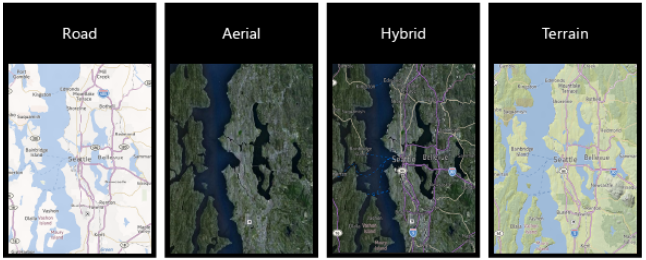
\includegraphics[scale=0.4]{Gambar/kartografi}
			\caption{\textit{Cartographic}}
			\label{fig:cartographic}
		\end{figure}
		
	\item	Mode warna yang disediakan Windows Phone ada dua yaitu terang dan gelap. Secara \textit{default} mode pada peta di Windows Phone adalah terang.
	
	\item Tampilan pada Peta di Windows Phone dapat berubah karena hasil diputar, dimiringkan, ditarik, dan diturunkan. Berikut beberapa hal yang dapat diatur sebagai tampilan di peta.
	
		\begin{itemize}
			\item \textit{Heading} merupakan representasi dari derajat secara geometri. Derajat ini didefinisikan dalam 0 sampai 360 yang dipakai untuk memutar peta. Contoh, 0 atau 360 ke arah utara, 90 ke arah barat, 180 ke arah selatan, dan 270 derajat ke arah timur.
			\item \textit{Pitch} merupakan derajat kemiringan dari peta dari sudut pengguna. Contoh, \textit{Pitch} = 0 berarti melihat dari atas ke bawah sedangkan \textit{Pitch} = 45 berarti melihat dari samping ke bawah dengan sudut 45 derajat.
		\end{itemize} 
\end{itemize}

% SUBSUB Pushpin ke Peta
\subsubsection{\textit{Pushpin} ke Peta}
\label{subsubsec:Pushpin ke Peta}
\hspace{0.5cm} \textit{Pushpin} merupakan elemen yang dapat ditempatkan pada peta secara spesifik dan bisa dipakai untuk interaksi pada peta. Peta tidak mendukung langsung penggunaan \textit{pushpin} karena merupakan elemen dari \textit{MapOverlay} (bagian/lapisan terpisah dari peta). Untungnya di Windows Phone memiliki Windows Phone 8 \textit{Toolkit} yang memiliki set objek agar dapat menggunakan \textit{pushpin} pada peta di Windows Phone. Contoh keluaran \textit{pushpin} dapat dilihat pada Gambar~\ref{fig:toolkit_pushpin} dan kode untuk menampilkannya dapat dilihat pada \textit{listing}~\ref{lst:pushpin}.

\begin{figure}[h]
	\centering
		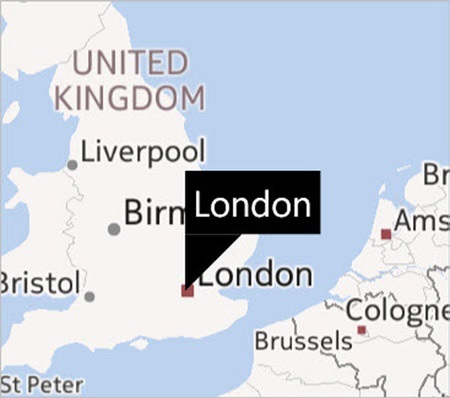
\includegraphics[scale=0.5]{Gambar/toolkit_pushpin}
	\caption{Keluaran Toolkit Pushpin pada Peta \cite{Manning}}
	\label{fig:toolkit_pushpin}
\end{figure}

\begin{lstlisting} [caption= {Kode untuk Menampilkan Pushpin},label={lst:pushpin}]
	MapOverlay overlay = new MapOverlay
	{
		GeoCoordinate = map.Center,
		Content = new Border
		{
		BorderBrush = new SolidColorBrush(Color.FromArgb(120, 255, 0, 0)),
		Child = new TextBlock(){Text="Pushpin"},
		BorderThickness = new Thickness(1),
		Background = new SolidColorBrush(Color.FromArgb(120,255,0,0)),
		Width = 80,
		Height = 60
		}
	};
	MapLayer layer = new MapLayer();
	layer.Add(overlay);

	map.Layers.Add(layer);
\end{lstlisting}

% SUBSUB Polyline pada Peta
\subsubsection{\textit{Polyline} pada Peta}
\label{subsubsec:Polyline pada Peta}
\hspace{0.5cm} Dalam menentukan arah dibutuhkan dua titik yaitu titk awal dan titik tujuan. Tentu saja arah tersebut butuh ditandai dengan garis. \textit{Polyline} merupakan tentetan garis lurus yang saling terhubung satu sama lain. Dengan \textit{polyline} arah pada peta dapat ditandai dengan warna maupin tebal atau tipisnya garis. Contoh keluaran \textit{polyline} dapat dilihat pada Gambar~\ref{fig:TampilanpolylinepadaPeta} dan kode untuk menampilkannya dapat dilihat pada \textit{listing}~\ref{lst:polyline}.

\begin{figure}[h]
	\centering
		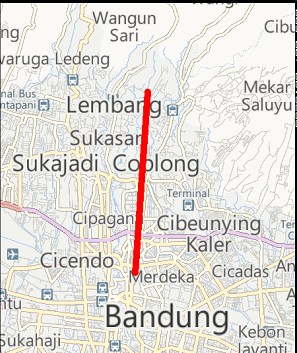
\includegraphics[scale=0.5]{Gambar/kontrol/polyline}
	\caption{Tampilan Polyline pada Peta}
	\label{fig:TampilanpolylinepadaPeta}
\end{figure}

\begin{lstlisting} [caption= {Kode untuk Menampilkan Polyline},label={lst:polyline}]
	MapPolyline line = new MapPolyline();
	line.StrokeColor = Colors.Red;
	line.StrokeThickness = 10;
	line.Path.Add(new GeoCoordinate(-6.8619546, 107.614441));
	line.Path.Add(new GeoCoordinate(-6.908693, 107.611185));
\end{lstlisting}

% SUBSUB Namespace Map
\subsubsection{\textit{Namespace Control Map}}
\label{subsubsec:Namespace Control Map}
\hspace{0.5cm} \textit{Namespace} merupakan nama yang dipakai untuk mengatur kelas-kelas. Windows Phone 8 sudah menyediakan \textit{namespace} bawaan untuk mengatur peta. \textit{Namespace} yang disediakan adalah \textit{Maps.Controls}. \textit{Namespace} ini yang berisi kelas-kelas yang paling sering digunakan untuk mengatur peta pada Windows Phone.  Agar dapat menggunakan kelas pada \textit{namespace} tersebut perlu ditambahkan \textit{namespace} dan \textit{capabilities}. \textit{Namespace} yang harus ditambahkan pada baris awal XAML adalah \textit{Microsoft.Phone.Maps.Controls}. Selanjutnya ada penambahan \textit{capabilities} \textit{ID\_CAP\_MAP}. Penambahan \textit{capabilities} ditambahkan pada \textit{WMAppManifest.xml}.

% SUBSUB Kelas Map
\subsubsection{Kelas Map}
\label{subsubsec:Kelas Map}
\hspace{0.5cm} Merupakan kelas yang mewakili kontrol map.

Berikut properti yang dapat digunakan pada kelas ini.
\begin{table}[h]
	\centering
		\begin{tabular}{ |c|c|}
				\hline
					Nama & Deskripsi \\ \hline
					\textit{CartographicMode} & Mengatur dan mendapatkan tipe dari peta. \\ \hline
					\textit{Center} & Mengatur dan mendapatkan titik tengah pada peta. \\ \hline
					\textit{ColorMode} & Mengatur dan mendapatkan mode warna peta. \\ \hline
					\textit{Heading} & Mengatur dan mendapatkan arah pandang peta. \\ \hline
					\textit{Height} & Mengatur dan mendapatkan tinggi. \\ \hline
					\textit{LandmarksEnabled} & Indikasi apakah bangunan 3D ditampilkan. \\ \hline
					\textit{Name} & Mengatur dan mendapatkan nama untuk identifikasi objek. \\ \hline
					\textit{PedestrianFeaturesEnabled} & Indikasi fitur pejalan kaki ditampilkan. \\ \hline
					\textit{Pitch} & Mengatur dan mendapatkan derajat kemiringan peta. \\ \hline
					\textit{Tag} & Mengatur dan mendapatkan nilai objek. \\ \hline
					\textit{TileSources} & Mendapatkan koleksi lapisan lantai. \\ \hline
					\textit{Width} & Mengatur dan mendapatkan lebar. \\ \hline
					\textit{ZoomLevel} & Mengatur dan mendapatkan tingkat zoom pada peta. \\ \hline
				\hline
		\end{tabular}
	\caption{Properti Kelas Map}
	\label{tab:PropertiKelasMap}
\end{table}

Berikut \textit{method} yang dapat digunakan pada kelas ini.
\begin{itemize}
	\item \textit{SetView(LocationRectangle)} \\
	\textit{method} untuk mengatur pandangan di atas peta secara spesifik sesuai wilayah geografis. \textit{method} ini tidak mengembalikan nilai.
	\item \textit{SetView(GeoCoordinate, Double)} \\
	\textit{method} untuk mengatur pandangan di atas peta secara spesifik sesuai titik tengah dan tingkat zoom. \textit{method} ini tidak mengembalikan nilai.
	\item \textit{SetView(LocationRectangle, MapAnimationKind)}\\
	\textit{method} untuk mengatur pandangan di atas peta secara spesifik sesuai region geografis dan animasi. \textit{method} ini tidak mengembalikan nilai.
	\item \textit{SetView(LocationRectangle, Thickness)} \\
	\textit{method} untuk mengatur pandangan di atas peta secara spesifik sesuai region geografis dengan batas tertentu. \textit{method} ini tidak mengembalikan nilai.
	\item \textit{SetView(GeoCoordinate, Double, MapAnimationKind)} \\
	\textit{method} untuk mengatur pandangan di atas peta secara spesifik sesuai titik tengah, tingkat zoom, dan animasi. \textit{method} ini tidak mengambalikan nilai.
	\item \textit{SetView(GeoCoordinate, Double, Double)} \\
	\textit{method} untuk mengatur pandangan di atas peta secara spesifik sesuai titik tengah, tingkat zoom, dan \textit{heading}. \textit{method} ini tidak mengembalikan nilai.
	\item \textit{SetView(LocationRectangle, Thickness, MapAnimationKind)} \\
	\textit{method} untuk mengatur pandangan di atas peta secara spesifik sesuai wilayah geografis dengan batas tertentu, dan animasi. \textit{method} ini tidak mengembalikan nilai.
	\item \textit{SetView(GeoCoordinate, Double, Double, MapAnimationKind)} \\
	\textit{method} untuk mengatur pandangan di atas peta secara spesifik sesuai titik tengah, tingkat zoom, \textit{heading}, dan animasi. \textit{method} ini tidak mengembalikan nilai.	
	\item \textit{SetView(GeoCoordinate, Double, Double, Double)} \\
	\textit{method} untuk mengatur pandangan di atas peta secara spesifik sesuai titik tengah, tingkat zoom, \textit{heading}, \textit{pitch}. \textit{method} ini tidak mengembalikan nilai.
	\item \textit{SetView(GeoCoordinate, Double, Double, Double, MapAnimationKind)} \\
	\textit{method} untuk mengatur pandangan di atas peta secara spesifik sesuai titik tengah, tingkat zoom, \textit{heading}, \textit{pitch}, dan animasi. \textit{method} ini tidak mengembalikan nilai.
	\item \textit{UpdateLayout} \\
	\textit{method} yang memastikan semua posisi objek turunan mengikuti tata letak. 
\end{itemize}

% SUBSUB Polyline Class
\subsubsection{\textit{Polyline Class}}
\label{subsubsec:Polyline Class}
\hspace{0.5cm} Merupakan kelas yang dipakai untuk menggambarkan garis lurus yang saling terhubung. Kelas ini tergabung ke dalam \textit{namespace Microsoft.Phone.Maps.Controls}. 
\newpage
Berikut properti yang dapat digunakan pada kelas ini.
\begin{table}[h]
	\centering
		\begin{tabular}{ |p{4cm}|p{10cm}|}
				\hline
					Nama & Deskripsi \\ \hline
					\textit{Dispacher} & Mendapatkan objek yang terkait. \\ \hline
					\textit{Path} & Mengatur dan mendapatkan kumpulan nilai \textit{GeoCoordinates} yang membuat \textit{polyline}. \\ \hline
					\textit{StrokeColor} & Mengatur dan mendapatkan warna garis. \\ \hline
					\textit{StrokeDashed} & Mengatur dan mendapatkan nilai untuk menggambar \textit{polyline} pustus-putus. \\ \hline
					\textit{StrokeThickness} & Mengatur dan mendapatkan lebar garis untuk menggambar \textit{polyline}. \\ \hline
				\hline
		\end{tabular}
	\caption{Properti \textit{Polyline Class}}
	\label{tab:PropertiKelasPolyline}
\end{table}

Berikut \textit{method} yang dapat digunakan pada kelas ini.
\begin{itemize}
	\item \textit{CheckAccess}\\
	\textit{method} yang menentukan bisa atau tidaknya pemanggilan \textit{thread} untuk mengakses objek.
	\item \textit{ClearValue}\\
	\textit{method} yang akan membersihkan nilai lokal
	\item \textit{Finalize} \\
	\textit{method} yang dipakai untuk melakukan pembersihan pada sumber daya yang tidak terpakai sebelum objek dihancurkan.
\end{itemize}

% SUBSUB Pushpin Class
\subsubsection{\textit{Pushpin Class}}
\label{subsubsec:Pushpin Class}
\hspace{0.5cm} Merupakan kelas yang dipakai untuk menggambarkan elemen terpisah diatas peta. Meskipun pushpin merupakan bawaan pada peta untuk menunjuk suatu lokasi tetapi \textit{pushpin} dari peta tidak dapat diubah-ubah. \textit{Pushpin} pada Windows Phone 8 dapat dibuat sesuai kebutuhan. Namun ada cara lain dengan menambahkan Windows Phone Toolkit. Windows Phone Toolkit mempunyai komponan untuk menggambar pushpin diatas peta.  
%sumber http://developer.nokia.com/resources/library/Lumia/change-history/archived-content/maps-and-navigation/guide-to-the-wp8-maps-api.html

% SUB Lokasi
\subsection{Lokasi}
\label{subsec:Lokasi}
\hspace{0.5cm} Aplikasi di Windows Phone 8 dapat memanfaatkan lokasi di mana perangkat berada. Aplikasi dapat melacak lokasi sesaat  pengguna atau pelacakan selama periode tertentu. Data lokasi perangkat berasal dari berbagai sumber termasuk \textit{Global Positioning System} (GPS), \textit{Wireless Fidelity} (Wi-Fi), dan jaringan seluler. Ada 2 set API berbeda yang dapat dimanfaatkan di Windows Phone yaitu \textit{Runtime Location} API dan .NET \textit{Location} API. Windows Phone \textit{Runtime Location} memiliki keunggulan fitur yang banyak sedangkan .NET \textit{Location} direkomendasikan jika aplikasi ditargetkan pada Windows Phone 7.1 dan Windows Phone 8\cite{MSDN}.

Hal yang perlu diperhatikan dalam menentukan layanan lokasi adalah penangkap GPS, Wi-Fi, dan jaringan seluler. Perangkat tersebut berfungsi sebagai penyedia data lokasi dengan berbagai tingkat akurasi dan konsumsi daya. Perangkat diatas juga berkomunikasi langsung untuk memutuskan sumber mana yang digunakan untuk menentukan lokasi perangkat berdasarkan ketersediaan data lokasi dan prasyarat yang ditentukan aplikasi. Lapisan diatas penyedia data lokasi tersebut adalah pengelola antarmuka. Aplikasi akan mengunakan antarmuka tersebut untuk memulai dan menghentikan layanan lokasi, mengatur tingkat akurasi, dan menerima data lokasi.

Karena pengguna dapat berpindah tempat untuk menuju tempat yang lain, maka pelacakan lokasi harus dilakukan terus menerus. Pelacakan lokasi secara terus menerus ini dapat dilakukan di depan maupun di belakang aplikasi Windows Phone 8. Pelacakan aplikasi di depan akan memungkinkan aplikasi melacak lokasi pengguna sekaligus melakukan perbaruan antarmuka. Jika pelacakan lokasi di belakang aplikasi maka tidak ada perubahan pada antarmuka namun pelacakan dilakuan secara terus menerus. Pelacakan yang terus menerus di belakang aplikasi akan membuat keadaan aplikasi cepat dipulihkan dari keadaan \textit{Dormant}.

% SUBSUB Mendapatkan Posisi Pengguna
\subsubsection{Mendapatkan Posisi Pengguna}
\label{subsubsec:Mendapatkan Posisi Pengguna}
\hspace{0.5cm} Di Windows Phone 8 telah ada \textit{GeoCoordinate class} yang dapat digunakan untuk mengetahui posisi pengguna. \textit{Geolocator class} dari \textit{Windows.Devices.Geolocation} akan mengembalikan posisi saat ini. Untuk menggunakan \textit{Geolocator}, perlu menghidupkan \textit{ID\_CAP\_LOCATION} di \url{/properties/WMAppManifest.xml}. Dalam mendapatkan posisi perlu diperhatikan status dari GPS karena membutuhkan waktu dari awal pengaktifan hingga mendapatkan lokasi pengguna secara akurat. Untuk lebih jelas mengenai status posisi dapat dilihat pada nilai status dibawah ini.

\begin{itemize}
	\item \textit{Ready} : Jika lokasi tersedia.
	\item \textit{Initializing} : Jika status penangkap GPS belum memiliki cukup satelit untuk mendapatkan posisi yang akurat. 
	\item \textit{NoData} : Data lokasi belum tersedia. Status ini muncul jika aplikasi sedang mamanggil \textit{GetGeopositionAsync()} atau \textit{register}.
	\item \textit{Disable} : Status mengindikasikan tidak diperbolehkannya pengaksesan lokasi.
	\item \textit{NotInitialized} : Data lokasi belum tersedia. Status ini muncul jika aplikasi belum mamanggil \textit{GetGeopositionAsync()} atau \textit{register}.
	\item \textit{NotAvailable} : Jika sensor arah mata angin dan lokasi tidak tersedia.
\end{itemize}

% SUBSUB Namespace Geolocator
\subsubsection{\textit{Namespace Geolocator}}
\label{subsubsec:Namespace Geolocator}
\hspace{0.5cm} \textit{Namespace} merupakan nama yang dipakai untuk mengatur kelas-kelas. Windows Phone 8 sudah menyediakan \textit{namespace} bawaan untuk mengakses lokasi. \textit{Namespace} yang disediakan adalah \textit{namespace geolocator}. \textit{Namespace} ini akan mengakses lokasi geografis dari perangkat dan mendukung pelacakan lokasi dari waktu ke waktu. Agar dapat menggunakan kelas pada \textit{namespace} tersebut perlu ditambahkan \textit{namespace} dan \textit{capabilities}. \textit{Namespace} yang harus ditambahkan pada baris awal XAML adalah \textbf{Windows.Device.Geolocator}. Selanjutnya ada penambahan \textit{capabilities ID\_CAP\_LOCATION}. Penambahan \textit{capabilities} ditambahkan pada \textit{WMAppManifest.xml}. Kelas yang diatur oleh \textit{namespace geolocator} dapat di lihat pada tabel ~\ref{tab:KelasPadaNamespaceGeolocator}\cite{DevWP8}.
\begin{table}[h]
	\centering
		\begin{tabular}{ |p{4cm}|p{10cm}|}
				\hline
				Kelas & Deskripsi \\ \hline
				\textit{Geocoordinate} & Berisi informasi untuk mengidentifikasi lokasi geografis. \\ \hline
				\textit{Geolocator} & Mendukung dalam pengaksesan lokasi perangkat. \\ \hline
				\textit{Geoposition} & Memberikan data lokasi beserta \textit{latitude} dan \textit{longitude} atau data alamat. \\ \hline
				\hline
		\end{tabular}
	\caption{Kelas pada \textit{Namespace Geolocator}}
	\label{tab:KelasPadaNamespaceGeolocator}
\end{table}

% SUBSUB Kelas Geocoordinate
\subsubsection{\textit{Geocoordinate}}
\label{subsubsec:Kelas Geocoordinate}
\hspace{0.5cm} Geocoordinate adalah kelas yang menunjukan lokasi sebagai kordinat geografis. Kelas ini hanya menyediakan properti yang hanya bisa dibaca. Kelas ini menyediakan properti yang ditunjukan pada tabel ~\ref{tab:PropertiPadaKelasGeocoordinate}.

\begin{table}[h]
	\centering
		\begin{tabular}{ |p{4cm}|p{10cm}|}
				\hline
				Properti & Deskripsi \\ \hline
				\textit{Altitude} & Ketinggian lokasi dalam satuan meter. \\ \hline
				\textit{Heading} & Arah menghadap perangkat dalam satuan derajat yang relative terhadap mata angin utara. \\ \hline
				\textit{Latitude} & Garis lintang dalam satuan derajat. \\ \hline
				\textit{Longitude}  & Garis bujur dalam satuan derajat. \\ \hline
				\textit{Point} & Lokasi dari \textit{Geocoordinate}. \\ \hline
				\textit{Speed} & Kecepatan dalam satuan meter per detik. \\ \hline
				\hline
		\end{tabular}
	\caption{Properti pada \textit{Geocoordinate}}
	\label{tab:PropertiPadaKelasGeocoordinate}
\end{table} 

% SUBSUB Kelas Geolocator
\subsubsection{\textit{Geolocator}}
\label{subsubsec:Kelas Geolocator}
\hspace{0.5cm} \textit{Geolocator} merupakan kelas yang mendukung pengaksesan terhadap lokasi.

Berikut \textit{method} yang disediakan \textit{Geolocator}:
\begin{itemize}
	\item \textit{public IAsyncOperation<Geoposition> GetGeopositionAsync()} \\
		Operator await diatas dimaksudkan untuk meminta posisi lokasi terus menerus sampai selesai dan menunda tugas yang lain. \\
		\textit{GetGeopositionAsync()} merupakan bawaan kelas \textit{Geolocator} akan meminta data lokasi dan menanganinya sampai selesai.
		Kembalian dari \textit{GetGeopositionAsync()} adalah objek \textit{Geoposition}.
\end{itemize}

Berikut Properti yang disediakan kelas Geolocator:
\begin{itemize}
	\item \textit{public PositionStatus LocationStatus} \{ get; \} \\
		Merupakan properti dari kelas \textit{geolocator} untuk mendapatkan status posisi dengan mengembalikan kelas \textit{PositionStatus}. Status pada kelas \textit{PositionStatus} adalah \textit{Ready}, \textit{Initializing}, \textit{NoData}, \textit{Disable}, \textit{NotInitialized}, dan \textit{NotAvailable}.
	\item \textit{public PositionAccuracy DesiredAccuracy} \{ get; set; \} \\
		Properti yang digunakan untuk mengatur dan mendapatkan tingkat akurasi. Untuk tingkat akurasi dapat dipilih tingkat \textit{High} untuk tingkat akurasi tinggi dan dipilih tingkat {Default} untuk menghemat daya. Keluaran dari properti ini adalah tipe data \textit{PositionAccuracy}.
	\item \textit{public Nullable<uint> DesiredAccuracyInMeters} \{ get; set; \}\\
		Sama seperti properti \textit{DesiredAccuracy} diatas tetapi dalam satuan meter. Keluaran dari properti ini adalah tipe data \textit{uint}.
	\item \textit{public uint ReportInterval} \{ get; set; \} \\
		Merupakan properti untuk mendapatkan selang waktu pembaruan lokasi. Properti ini mengeluarkan tipe data unit.
\end{itemize}

% SUBSUB Kelas Geoposition
\subsubsection{\textit{Geoposition}}
\label{subsubsec:Kelas Geoposition}
\hspace{0.5cm} \textit{Geoposition} merupakan kelas yang memuat lokasi (\textit{latitude} dan \textit{longitude}).
Berikut Properti yang disediakan kelas \textit{Geoposition}:
\begin{itemize}
	\item \textit{public CivicAddress CivicAddress} \{ get; \} \\
		Data alamat sipil yang terkait dengan lokasi geografis.
	\item \textit{public Geocoordinate Coordinate} \{ get; \} \\
		Data latitude dan longitude yang terkait lokasi geografis.
\end{itemize}

% SUB Memanfaatkan Sumber Data
\subsection{Memanfaatkan Sumber Data}
\label{subsec:Memanfaatkan Sumber Data}
\hspace{0.5cm} Hal yang penting dari sebuah aplikasi adalah informasi. Windows Phone 8 memiliki kemampuan dalam menghubungkan aplikasi dengan sumber data lainnya. Memanfaatkan sumber data ada dua cara yaitu yang lokal atau berada di perangkat dan \textit{web service}. \textit{Web Service} merupakan \textit{method} komunikasi antara dua perangkat melalui jaringan. 

Sebelum data dapat dikirim antar perangkat perlu dilakukan \textit{serialization}. \textit{Serialization} merupakan proses mentransformasikan objek ke format yang bisa dengan mudah dikirim melewati jaringan atau disimpan di database\cite{Manning}. Formatnya disini berupa string yang direpresentasikan sebagai objek di XML atau JSON(Javascript Object Notation). Setelah data yang dikirim didapatkan maka perlu dilakukan \textit{deserialization}. \textit{Deserialization} merupakan proses mentransformasikan dari format yang bisa dengan mudah dikirim melewati jaringan ke dalam bentuk objek. 

%sumber http://json.org/
Banyak \textit{web service} yang mengembalikan data dalam format JSON. JSON memiliki format \textit{data-interchange} yang ringan \cite{rfc7159}. Karena hal tersebut JSON mudah diurai dan dihasilkan oleh mesin. Kurung kurawal mengindikasikan objek, kurung siku berarti array, dan properti berupa nama dan nilai pasangan yang dipisahkan oleh titik dua. JSON format memiliki ukuran data yang kecil dan baik untuk penggunaan perangkat bergerak. Untuk contoh format JSON dapat dilihat di bagian Kiri API pada Bab dua ini karena Kiri API menggunakan format JSON. \textit{Serializes} menggunakan \textit{DataContractJsonSerializer} membuat \textit{serializes} mudah untuk menerjemahkan form String JSON ke objek yang dapat langsung digunakan. \textit{DataContractJsonSerializer} memakai \textit{WriteObject()} untuk \textit{serializes} and \textit{ReadObject()} untuk \textit{deserializes}.

% SUBSUB Kelas HttpClient
\subsubsection{\textit{HttpClient}}
\label{subsubsec:Kelas HttpClient}
\hspace{0.5cm} Merupakan Kelas yang dipakai untuk mengirim permintaan HTTP dan menerima kembalian HTTP dari \textit{Uniform Resource Identifier}(URI) yang dapat diidentifikasi. \textit{Uniform Resource Identifier}(URI) merupakan urutan kompak karakter yang mengidentifikasikan sumber daya abstrak dan fisik \cite{rfc3986}. Berikut \textit{method} yang disediakan kelas \textit{HttpClient}.
\begin{itemize}
	\item \textit{DeleteAsync(Uri)} \\
	\textit{method} yang dipakai untuk mengirimkan permintaan DELETE ke URI yang spesifik sebagai operasi \textit{asynchronous}. Maksud dari operasi \textit{asynchronous} adalah memungkinkan aplikasi untuk melanjutkan pekerjaan selagi \textit{method} ini dipanggil\footnotemark[2]. \textit{method} ini membutuhkan parameter URI sebagai tujuan dari permintaan. Sedangkan kembaliannya berupa objek yang mewakili operasi \textit{asynchronous} disertai kemajuan. Objek tersebut memiliki 2 parameter yaitu hasil berupa pesan kembalian dari http dan kemajuan dari data yang dikirim.
	\item \textit{GetAsync(Uri)} \\
	\textit{method} yang dipakai untuk mengirimkan permintaan \textit{GET} ke URI yang spesifik sebagai operasi \textit{asynchronous}. Maksud dari operasi \textit{asynchronous} adalah memungkinkan aplikasi untuk melanjutkan pekerjaan selagi \textit{method} ini dipanggil\footnotemark[2]. \textit{method} ini membutuhkan parameter URI sebagai tujuan dari permintaan. Sedangkan kembaliannya berupa objek yang mewakili operasi \textit{asynchronous} disertai kemajuan. Objek tersebut memiliki 2 parameter yaitu hasil berupa pesan kembalian dari http dan kemajuan dari data yang dikirim.
	\item \textit{GetAsync(Uri,HttpCompletionOption)} \\
	\textit{method} yang dipakai untuk mengirimkan permintaan \textit{GET} ke URI yang spesifik sebagai operasi \textit{asynchronous}. Maksud dari operasi \textit{asynchronous} adalah memungkinkan aplikasi untuk melanjutkan pekerjaan selagi \textit{method} ini dipanggil\footnotemark[2]. \textit{method} ini membutuhkan parameter URI sebagai tujuan dari permintaan dan nilai tambahan yang dimaksukan sebagai indikasi operasi dianggap selesai. Sedangkan kembaliannya berupa objek yang mewakili operasi \textit{asynchronous} disertai kemajuan. Objek tersebut memiliki 2 parameter yaitu hasil berupa pesan kembalian dari http dan kemajuan dari data yang dikirim.
	\item \textit{GetBufferAsync(Uri)} \\
	\textit{method} yang dipakai untuk mengirimkan permintaan \textit{GET} ke URI yang spesifik sebagai operasi \textit{asynchronous}. Maksud dari operasi \textit{asynchronous} adalah memungkinkan aplikasi untuk melanjutkan pekerjaan selagi \textit{method} ini dipanggil\footnotemark[2]. \textit{method} ini membutuhkan parameter URI sebagai tujuan dari permintaan. Sedangkan kembaliannya berupa objek yang mewakili operasi \textit{asynchronous} disertai kemajuan. Objek tersebut memiliki 2 parameter yaitu hasil berupa pesan kembalian yang dikirimkan secara buffer(disimpan dalam memori) dan kemajuan dari data yang dikirim.
	\item \textit{GetInputStreamAsync(Uri)} \\
	\textit{method} yang dipakai untuk mengirimkan permintaan \textit{GET} ke URI yang spesifik sebagai operasi \textit{asynchronous}. Maksud dari operasi \textit{asynchronous} adalah memungkinkan aplikasi untuk melanjutkan pekerjaan selagi \textit{method} ini dipanggil\footnotemark[2]. \textit{method} ini membutuhkan parameter URI sebagai tujuan dari permintaan. Sedangkan kembaliannya berupa objek yang mewakili operasi \textit{asynchronous} disertai kemajuan. Objek tersebut memiliki 2 parameter yaitu hasil berupa pesan kembalian yang dikirimkan secara stream(langsung sesuai waktu) dan kemajuan dari data yang dikirim.
	\item \textit{GetStringAsync(Uri)} \\
	\textit{method} yang dipakai untuk mengirimkan permintaan \textit{GET} ke URI yang spesifik sebagai operasi \textit{asynchronous}. Maksud dari operasi \textit{asynchronous} adalah memungkinkan aplikasi untuk melanjutkan pekerjaan selagi \textit{method} ini dipanggil\footnotemark[2]. \textit{method} ini membutuhkan parameter URI sebagai tujuan dari permintaan. Sedangkan kembaliannya berupa objek yang mewakili operasi \textit{asynchronous} disertai kemajuan. Objek tersebut memiliki 2 parameter yaitu hasil berupa pesan kembalian dalam bentuk string dan kemajuan dari data yang dikirim.
	\item \textit{PostAsync(Uri)} \\
	\textit{method} yang dipakai untuk mengirimkan permintaan \textit{POST} ke URI yang spesifik sebagai operasi \textit{asynchronous}. Maksud dari operasi \textit{asynchronous} adalah memungkinkan aplikasi untuk melanjutkan pekerjaan selagi \textit{method} ini dipanggil\footnotemark[2]. \textit{method} ini membutuhkan parameter URI sebagai tujuan dari permintaan. Sedangkan kembaliannya berupa objek yang mewakili operasi \textit{asynchronous} disertai kemajuan. Objek tersebut memiliki 2 parameter yaitu hasil berupa pesan kembalian dari http dan kemajuan dari data yang dikirim.
	\item \textit{SendRequestAsync(HttpRequestMessage)} \\
	\textit{method} yang dipakai untuk mengirimkan permintaan HTTP sebagai operasi \textit{asynchronous}. Maksud dari operasi \textit{asynchronous} adalah memungkinkan aplikasi untuk melanjutkan pekerjaan selagi \textit{method} ini dipanggil\footnotemark[2]. \textit{method} ini membutuhkan parameter pesan dari permintaan. Sedangkan kembaliannya berupa objek yang mewakili operasi \textit{asynchronous} disertai kemajuan. Objek tersebut memiliki 2 parameter yaitu hasil berupa pesan kembalian dari http dan kemajuan dari data yang dikirim.
	\item \textit{SendRequestAsync(HttpRequestMessage, HttpCompletionOption)} \\
	\textit{method} yang dipakai untuk mengirimkan permintaan HTTP sebagai operasi \textit{asynchronous}. Maksud dari operasi \textit{asynchronous} adalah memungkinkan aplikasi untuk melanjutkan pekerjaan selagi \textit{method} ini dipanggil\footnotemark[2]. \textit{method} ini membutuhkan parameter pesan dari permintaan dan nilai tambahan yang dimaksukan sebagai indikasi operasi dianggap selesai. Sedangkan kembaliannya berupa objek yang mewakili operasi \textit{asynchronous} disertai kemajuan. Objek tersebut memiliki 2 parameter yaitu hasil berupa pesan kembalian dari http dan kemajuan dari data yang dikirim.
\end{itemize}

\footnotetext[2]{\url{http://msdn.microsoft.com/en-us/library/ms734701\%28v=vs.110\%29.aspx}}
% http://msdn.microsoft.com/en-us/library/windows/apps/xaml/dn440594.aspx
% http://msdn.microsoft.com/en-us/library/windows/apps/xaml/windows.web.http.httpclient.aspx

% SUBSUB Json.NET from http://www.newtonsoft.com/json
\subsubsection{Json.NET}
\label{subsubsec:Json.NET}
\hspace{0.5cm} Json.NET merupakan \textit{library} untuk melakukan \textit{serialize} dan \textit{deserialize} terhadap objek dalam .NET \cite{jsonNet}. \textit{Library} ini memiliki 2 kelas yaitu kelas JsonConvert dan kelas JsonSerializer. Berikut merupakan keterangan dari dua kelas tersebut.
\begin{itemize}
	\item Kelas JsonConvert merupakan kelas yang dapat mengkonversi objek ke JSON dalam bentuk String dan sebaliknya. Berikut 2 buah \textit{method} yang disediakan kelas JsonConvert. \\
		\begin{enumerate}
			\item \textit{Method} SerializeObject() \\
			\textit{Method} yang dipakai untuk mengkonversi objek ke JSON dalam bentuk String.
			\item \textit{Method} DeserializeObject()\\
			\textit{Method} yang dipakai untuk mengkonversi JSON dalam bentuk String ke objek.
		\end{enumerate}
	\item Kelas JsonSerializer merupakan kelas yang dapat melakukan \textit{serializes} dan \textit{deserializes} objek ke dan dari JSON format.
\end{itemize}

% SUB Thread
% from https://msdn.microsoft.com/en-us/library/windows/desktop/ms681917(v=vs.85).aspx
\subsection{Thread}
\label{subsec:Thread}
\hspace{0.5cm} Thread merupakan entitas dalam suatu proses yang dapat dijalankan untuk eksekusi sebuah operasi. 

\subsubsection{\textit{BackgroundWorker}}
\label{subsubsec:BackgroundWorker}
\hspace{0.5cm} \textit{BackgroundWorker} merupakan kelas dari Windows Phone yang dapat mengeksekusi operasi dalam thread terpisah. Berikut \textit{method} yang disediakan kelas \textit{BackgroundWorker}.
\begin{itemize}
	\item \textit{RunWorkerAsync()} \\
	\textit{method} yang digunakan untuk memulai eksekusi operasi di latar belakang.
\end{itemize}

Berikut \textit{event} yang disediakan kelas \textit{BackgroundWorker}.
\begin{itemize}
	\item \textit{DoWork} \\
	\textit{event} yang terjadi ketika \textit{method RunWorkerAsync()} dipanggil.
	\item \textit{RunWorkerCompleted} \\
	\textit{event} yang terjadi ketika operasi di latar belakang selesai dilakukan, dibatalkan, atau mencapai \textit{exception}.
\end{itemize}

% Kiri API
\section{Kiri API}
\label{sec:Kiri API}
\hspace{0.5cm} API atau \textit{Application Programming Interface} merupakan aturan yang dikodekan secara spesifik yang dapat digunakan untuk komunikasi antar aplikasi. Jadi API disini memfasilitasi untuk pemanggilan fungsi-fungsi tertentu diluar aplikasi itu sendiri. Pemanfaatan Kiri API dilakukan dengan menggunakan JSON atau \textit{JavaScript Object Notation} format. 

Pemanfaatan Kiri API dengan melakuan permintaan dengan parameter \textit{POST} atau \textit{GET} lalu Kiri akan mengembalikan hasil dalam format JSON. Permintaan tersebut dikirimkan ke URL atau \textit{Uniform Resource Locator}. Berikut URL yang disediakan Kiri Api.
\begin{itemize}
	\item \url{http://preview.kiri.travel/handle.php} \\
	Merupakan URL untuk uji coba. Untuk kemampuannya juga menurut dokumentasi Kiri API masih tidak stabil.
	\item \url{http://kiri.travel/handle.php} \\
	Merupakan URL produksi. Ini merupakan URL yang direkomendasikan untuk menangani permintaan pengguna.
\end{itemize}
Untuk setiap permintaan membutuhkan \textit{API key} yang didapat dengan mendaftar\cite{Kiri}. Penggunaan API memungkinkan pengaksesan di mana saja dengan menggunakan koneksi internet. Pada sub bab~\ref{subsec:Web Service Penentuan Rute} sampai sub bab~\ref{subsec:Service Menemukan Transportasi Terdekat} penulis akan membahas beberapa layanan Kiri API.

Berikut langkah-langkah untuk mendapatkan \textit{API key}.
\begin{itemize}
	\item Masuk ke situs \url{dev.kiri.travel}.
	\item Register dengan memasukan alamat email, nama, dan nama perusahaan.
	\item Password akan dikirimkan ke alamat email. Tentunya password akan dibuat otomatis oleh pihak Kiri.
	\item Login dengan menggunakan password yang dikirim ke alamat email. 
	\item Setelah berhasil login, di menu utama pilih \textit{API Keys Managements}.
	\item Pilih tombol Add lalu masukan deskripsi penggunaan \textit{API key}.
	\item \textit{API key} didapat dan dapat digunakan.
\end{itemize}

% SUB Web Service Penentuan Rute
\subsection{\textit{Web Service} Penentuan Rute}
\label{subsec:Web Service Penentuan Rute}
\hspace{0.5cm} \textit{Web service} penentuan rute merupakan layanan Kiri API yang digunakan untuk mendapatkan langkah perjalanan dari lokasi asal ke lokasi tujuan. Parameter dan keterangan untuk layanan ini dapat dilihat pada tabel~\ref{tab:routingWebService}.

\begin{table}[H]
	\centering
		\begin{tabular}{|p{2cm}|p{4cm}|p{8cm}|}
			\hline
			\textit{version} & 2 & Memberitahukan bahwa layanan yang \strut dipakai adalah protokol veris 2 \\ \hline
			\textit{mode} & "findroute" & Mengintruksikan layanan untuk mencari rute \\ \hline
			\textit{locale} & "en" or "id" & Bahasa yang digunakan untuk balasan \\ \hline
			\textit{start} & lat,lng & Titik awal \textit{latitude} dan \textit{longitude} \\ \hline
			\textit{finish} & lat,lng & Titik akhir \textit{latitude} dan \textit{longitude}  \\ \hline
			\textit{presentation} & "mobile" or "desktop" & Menentukan tipe presentasi untuk keluaran. Contoh, jika tipe presentasi "mobile", maka link "tel:" akan ditambahkan di hasil. \\ \hline
			\textit{apikey} & 16-digit hexadecimals & \textit{API key} yang digunakan \\ \hline
			\hline
		\end{tabular}
	\caption{Tabel Parameter Layanan Penentuan Rute}
	\label{tab:routingWebService}
\end{table}

Format kembalian layanan penentuan rute dapat dilihat pada \textit{listing}~\ref{lst:pencarian}:

\begin{lstlisting} [caption= {Kode Kembalian Pencarian Rute},label={lst:pencarian}]
{ 
    "status": "ok" or "error" 
    "routingresults": [ 
        {
            "steps": [
                [
                    "walk" or "none" or others,
                    "walk" or vehicle_id or "none",
                    ["lat_1,lon_1", "lan_2,lon_2", ... "lat_n,lon_n"],
                    "human readable description, dependant on locale",
                    URL for ticket booking or null (future)
                ],
                [
                    "walk" or "none" or others,
                    "walk" or vehicle_id or "none",
                    ["lat_1,lon_1", "lan_2,lon_2", ... "lat_n,lon_n"],
                    "human readable description, dependant on locale",
                    URL for ticket booking or null (future)
                ]
            ],
            "traveltime": any text string, null if and only if route is not found.
        } ,
        {
            "steps": [ ... ],
            "traveltime": "..."
        } ,
        {
            "steps": [ ... ],
            "traveltime": "..."
        } ,
        ...     
    ]
}
\end{lstlisting}
Berikut maksud dari \textit{listing}~\ref{lst:pencarian}: \newline
\hspace{0.5cm} Ketika pencarian rute sukses dilakukan maka status akan memberitahukan "ok" seperti di baris 2. Selanjutnya setiap langkah dari posisi awal ke posisi tujuan akan ditampung di elemen \textit{array} untuk menampung langkah. Berikut keterangan dari setiap \textit{array} yang menampung langkah. 

\begin{itemize}
	\item Indeks ke 0 atau baris 7 pada \textit{listing}~\ref{lst:pencarian} dapat berisi "walk" atau "none" atau "others". Baris tersebut berarti jika "walk" untuk berjalan kaki, "none" jika rute tidak ditemukan dan "others" untuk menggunakan kendaran.
	\item Indeks ke 1 atau baris 8 pada \textit{listing}~\ref{lst:pencarian} merupakan detail dari indeks 0. Artinya jika indeks 0 menyatakan "walk" berarti indeks 1 harus "walk", "none" berarti indeks 1 harus "none", dan selain itu menyatakan id kendaraan yang mana bisa dipakai untuk ditampilkan gambarnya.
	\item Indeks ke 2 atau baris 9 pada \textit{listing}~\ref{lst:pencarian} adalah deretan nilai tipe \textit{String} yang berisi jalur dalam format "lat,lng". Maksud dari "lat,lng" disini adalah titik awal dan titik akhir dari setiap jalur yang dilewati.
	\item Indeks ke 3 atau baris 10 pada \textit{listing}~\ref{lst:pencarian} berisi bentuk yang akan ditampilkan kepada pengguna. Informasi yang disampaikan dapat berupa:
		\begin{itemize}
			\item \%fromicon = untuk menunjukan ikon "from". Biasanya untuk mode presentasi di perangkat bergerak.
			\item \%toicon = untuk menunjukan ikon "to". Biasanya untuk mode presentasi di perangkat bergerak. 
		\end{itemize}
	\item Indeks ke 4 atau bari 11 pada \textit{listing}~\ref{lst:pencarian} berisi URL untuk pemesanan tiket jika tersedia. Jika tidak tersedia akan bernilai \textit{null}.
\end{itemize}

\hspace{0.5cm} Kiri telah menyediakan gambar untuk setiap angkutan umum. Gambar tersebut dapat di akses di URL:
\begin{itemize}
	\item \url{http://kiri.travel/images/means/[means]/[means_details].png}
	\item \url{http://kiri.travel/images/means/[means]/baloon/[means_details].png}
\end{itemize}
Nilai [means] dapat diambil dari indeks 0 nilai kembalian dan nilai [means\_details] dapat diambil dari indeks 1 nilai kembalian. 
		
% SUB Web Service Pencarian Lokasi
\subsection{\textit{Web Service} Pencarian Lokasi}
\label{subsec:Pencarian Lokasi Service}
\hspace{0.5cm} Merupakan layanan Kiri API yang digunakan untuk mencari lokasi beserta kordinat \textit{latitude} dan \textit{longitude}. Parameter dan keterangan untuk layanan ini dapat dilihat pada tabel~\ref{tab:pencarianLokasi}.

\begin{table}[H]
	\centering
		\begin{tabular}{ |p{2cm}|p{4cm}|p{8cm}| }
			\hline
			\textit{version} & 2 & Memberitahukan bahwa layanan yang dipakai adalah protokol veris 2 \\ \hline
			\textit{mode} & "searchplace" & Mengintruksikan layanan untuk mencari tempat \\ \hline
			\textit{region} & "cgk" or "bdo" or "sub" & Kota yang akan dicari tempatnya \\ \hline
			\textit{querystring} & teks apa saja dengan minimum text satu karakter & \textit{Query string} yang akan dicari menggunakan  layanan ini \\ \hline
			\textit{apikey} & 16-digit heksadesimal & \textit{API key} yang digunakan \\ \hline
			\hline
		\end{tabular}
	\caption{Tabel Parameter Layanan Pencarian Lokasi}
	\label{tab:pencarianLokasi}
\end{table}

\vspace{5mm}
Format kembalian dari layanan pencarian lokasi dapat dilihat pada \textit{listing}~\ref{lst:pencarianLokasi}.

\begin{lstlisting} [caption= {Kode Lembalian Pencarian Lokasi},label={lst:pencarianLokasi}]
{
    "status": "ok" or "error"
    "searchresult": [
        {
            "placename": "place name"
            "location": "lat,lon"
        },
        {
            "placename": "place name"
            "location": "lat,lon"
        },
        ...
    ]
    "attributions": [
        "attribution_1", "attribution_2", ...
    ]
}
\end{lstlisting}
Berikut maksud dari \textit{listing}~\ref{lst:pencarianLokasi}: 
\newline
\hspace{0.5cm} Ketika pencarian lokasi sukses dilakukan maka status akan memberitahukan "ok" seperti di baris 2. Selanjutnya akan ditampilkan hasil dari lokasi yang ada beserta atributnya. Berikut keterangan dari format dari pencarian lokasi:
\begin{itemize}
	\item "searchresult"' (pada baris 4 sampai 7, 8 sampai 11, dan seterusnya) berisi array dari tempat:
	\begin{itemize}
		\item placename: nama tempat
		\item location: latitude dan longitude dari tempat
	\end{itemize}
	\item "attributions" berisi kumpulan nilai yang berisikan atribut tambahan untuk dimunculkan.
\end{itemize}	

% SUB Web Service Memilih Transportasi Terdekat
\subsection{\textit{Web Service} Menemukan Transportasi Terdekat}
\label{subsec:Service Menemukan Transportasi Terdekat}
\hspace{0.5cm} Merupakan Kiri API yang digunakan untuk menemukan rute transportasi terdekat sesuai titik yang diinginkan pengguna. Parameter dan keterangan untuk layanan ini dapat dilihat pada tabel~\ref{tab:transportasiTerdekat}.

\begin{table}[H]
	\centering
		\begin{tabular}{ |p{2cm}|p{4cm}|p{8cm}| }
			\hline
			\textit{version} & 2 &  Memberitahukan bahwa layanan yang dipakai adalah protokol veris 2 \\ \hline
			\textit{mode} & "nearbytransports" & Mengintruksikan layanan untuk mencari rute transportasi terdekat \\ \hline
			\textit{start} & \textit{latitude} dan \textit{longitude} & Kota yang akan dicari tempatnya \\ \hline
			\textit{apikey} & 16-digit hexadesimal & \textit{API key} yang digunakan \\ \hline
			\hline
		\end{tabular}
	\caption{Tabel Parameter :ayanan Menemukan Transportasi Terdekat}
	\label{tab:transportasiTerdekat}
\end{table}


Format kembalian layanan menemukan transportasi terdekati dapat dilihat pada \textit{listing}~\ref{lokasiTerdekat}.

\begin{lstlisting} [caption= {Kode Kembalian Menemukan Lokasi Terdekat},label={lokasiTerdekat}]
{
    "status": "ok" or "error"
    "nearbytransports": [
        [
            "walk" or "none" or others,
            "walk" or vehicle_id or "none",
            text string,
            decimal value
        ],
        [
            "walk" or "none" or others,
            "walk" or vehicle_id or "none",
            text string,
            decimal value
        ],
        ...     
    ]
}\end{lstlisting}
Berikut maksud dari \textit{listing}~\ref{lokasiTerdekat}: \newline
\hspace{0.5cm} Ketika pencarian rute sukses dilakukan maka status akan memberitahukan "ok" seperti di baris 2. Selanjutnya akan diberikan array yang berisi transportasi terdekat yang diurutkan dari yang terdekat ke yang terjauh. Berikut keterangan dari setiap array tersebut: 
\begin{itemize}
	\item Indeks ke 0 atau baris 5 pada \textit{listing}~\ref{lokasiTerdekat} dapat berisi "walk" atau "none" atau "others". Artinya  jika "walk" berarti berjalan kaki, "none" jika rute tidak ditemukan dan "others" berarti menggunakan kendaran.
	\item Indeks ke 1 atau baris 6 pada \textit{listing}~\ref{lokasiTerdekat} merupakan detail dari indeks 0. Artinya jika indeks 0 "walk" berarti indeks 1 harus "walk", "none" berarti indeks 1 harus "none" dan selain itu menyatakan id kendaraan yang mana bisa dipakai untuk ditampilkan gambarnya.
	\item Indeks ke 2 atau baris 7 pada \textit{listing}~\ref{lokasiTerdekat} berisi nama kendaraan.
	\item Indeks ke 3 atau baris 8 pada \textit{listing}~\ref{lokasiTerdekat} berisi jarak dengan satuan kilometer.
\end{itemize}